\documentclass[conference]{IEEEtran}
\IEEEoverridecommandlockouts

% Packages
\usepackage{amsmath,amssymb}
\usepackage{graphicx}
\usepackage{url}
\usepackage{hyperref}

% Title
\title{
MeshGuardian: The Unbreakable Thread of Tomorrow�s Communication
}

% Author
\author{
    \IEEEauthorblockN{Chokri Mahmoud}
    \IEEEauthorblockA{
        Email: \texttt{acutclub@gmail.com} \\
        Affiliation: Independent Researcher \\
        GitHub: \url{https://github.com/macleen/meshguardian}
    }
}

\begin{document}
\maketitle

% Abstract
\begin{abstract}
When the world goes silent�cut off by storms, stranded in space, or lost in the wild�MeshGuardian speaks. Built for Delay-Tolerant Networks (DTNs), it�s not just a protocol; it�s a rebellion against the limits of today�s communication. Where others falter with weak security, bloated energy demands, or rigid designs, MeshGuardian soars with post-quantum shields, AI-powered agility, and a whisper-light footprint. This is the future, woven into every byte.
\end{abstract}

% Keywords
\begin{IEEEkeywords}
DTN, mesh networks, synchronization, blockchain audit, post-quantum cryptography, AI optimization, energy efficiency, interplanetary networking
\end{IEEEkeywords}

% Introduction
\section{Introduction: A Beacon in the Dark}
Picture this: a city drowned by a tsunami, its towers toppled, its people desperate. A rover on Mars, millions of miles from help, clutching data that could rewrite science. A farmer in a desert, cut off, yet holding the key to a global breakthrough. Traditional networks�TCP/IP, Wi-Fi�collapse here like sandcastles against the tide. Even DTN veterans like the Bundle Protocol limp along, shackled by outdated security and clunky scalability. MeshGuardian doesn�t just step in�it storms the stage, rewriting the rules with a protocol that�s as tough as titanium and as clever as a fox.

Why settle for flickering candles when you can wield a lighthouse? MeshGuardian outshines the competition with:
\begin{itemize}
    \item \textbf{Unmatched Security}: Post-quantum cryptography laughs at tomorrow�s threats.
    \item \textbf{Scalability on Steroids}: From a lone sensor to a galaxy-spanning fleet.
    \item \textbf{Energy Wizardry}: Sips power where others guzzle.
    \item \textbf{Adaptability}: A chameleon in a world of rigid relics.
\end{itemize}

% Related Work
\section{Related Work: Giants with Clay Feet}
The old guard of DTN and mesh networking�Bundle Protocol, B.A.T.M.A.N., OLSR�try hard, but they�re no match for MeshGuardian�s brilliance. The Bundle Protocol, a spacefaring pioneer, chokes on high latency and offers no armor against quantum hacks. B.A.T.M.A.N. and OLSR, terrestrial titans, buckle under extreme delays and power-hungry designs. MeshGuardian doesn�t just compete�it redefines the battlefield:

\begin{itemize}
    \item \textbf{Security Edge}: While others wield rusty locks, MeshGuardian brandishes a quantum-proof vault.
    \item \textbf{Efficiency Leap}: Nano-sync packets dance where others trudge with heavy payloads.
    \item \textbf{AI Smarts}: Predictive optimizations outwit static routing every time.
    \item \textbf{Trust Revolution}: Blockchain audit trails leave centralized faith in the dust.
\end{itemize}

\begin{figure}[h]
    \centering
    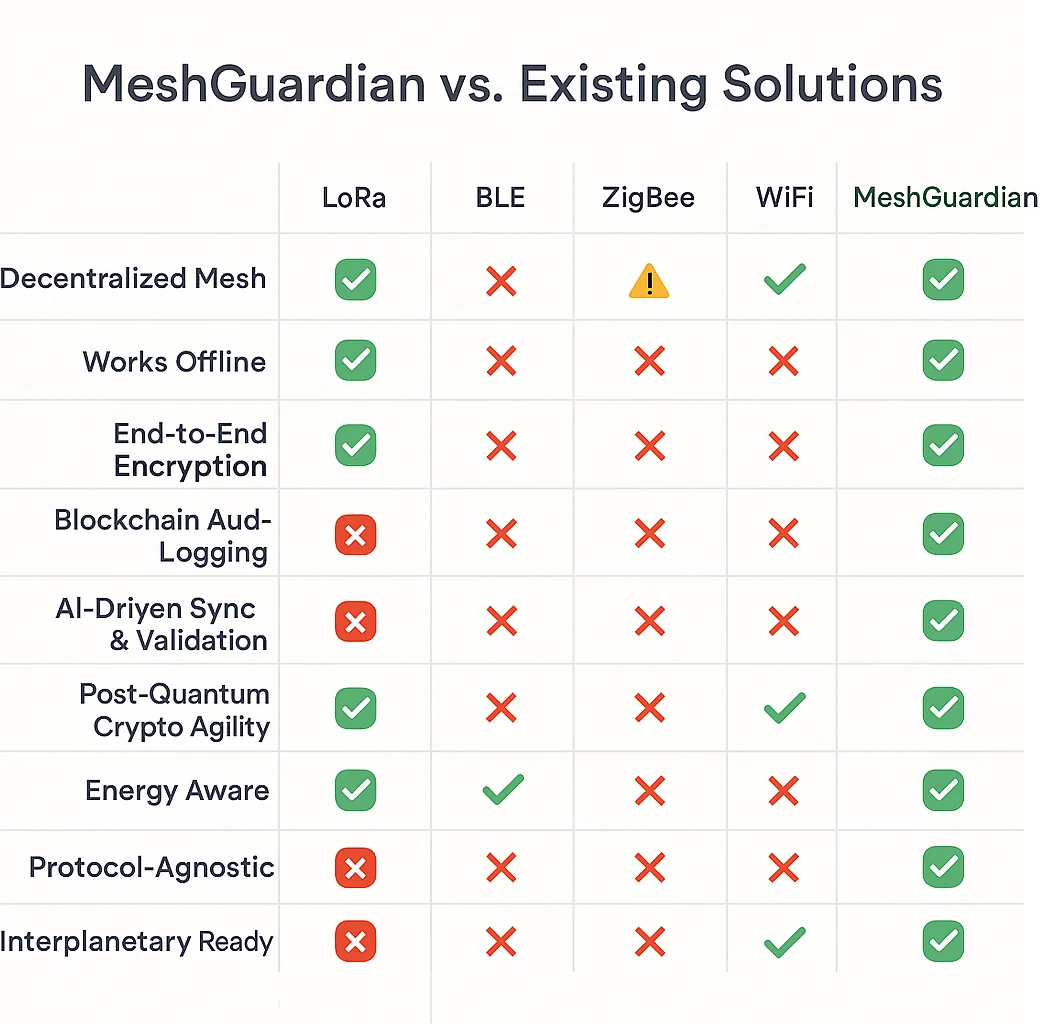
\includegraphics[width=0.8\linewidth]{comparison_chart.png}
    \caption{MeshGuardian vs. the Old Guard}
    \label{fig:comparison_chart}
\end{figure}

% Design Principles
\section{Design Principles: The Pillars of a Titan}
MeshGuardian stands on a foundation no storm can shake:
\begin{itemize}
    \item \textbf{Resilience}: Laughs at disconnection, dances THROUGH delays.
    \item \textbf{Security}: AES-256, Schnorr signatures, and Kyber-Dilithium�unbreakable today, invincible tomorrow.
    \item \textbf{Scalability}: A whisper to a swarm, effortlessly.
    \item \textbf{Auditability}: Every byte etched in blockchain stone�tamper-proof forever.
    \item \textbf{Modularity}: A Pluggable Protocol Engine that bends like bamboo, never breaks.
    \item \textbf{Energy Mastery}: Runs on crumbs while others feast.
\end{itemize}

% Packet Structure
\section{Packet Structure: A Masterpiece in Miniature}
Every MeshGuardian packet is a tiny warrior:
\begin{itemize}
    \item \textbf{Header (128 bytes)}: The strategist�routing, timestamps, flags sharp as a blade.
    \item \textbf{Payload}: The soul�encrypted tight, compressed lean, PrivacySafePod cloaking secrets.
    \item \textbf{Trailer (96 bytes)}: The sentinel�signatures and audit hashes standing guard.
\end{itemize}

\begin{figure}[h]
    \centering
    \includegraphics[width=0.8\linewidth]{packet_structure.png}
    \caption{The MeshGuardian Packet Unveiled}
    \label{fig:packet_structure}
\end{figure}

% Synchronization Mechanism
\section{Synchronization: A Symphony Across the Void}
Imagine a choir singing in perfect harmony, voices separated by oceans yet flawlessly aligned. That�s MeshGuardian�s sync engine. With offline buffering, Lamport timestamps, and nano-sync packets (a mere 10 bytes!), it turns chaos into clockwork. Vector clocks and conflict arbitration weave a tapestry of consistency, no matter how fierce the storm.

% Consensus Engine
\section{Consensus: The Heartbeat of Trust}
MeshGuardian�s hybrid consensus is a marvel of balance:
\begin{itemize}
    \item \textbf{Proof-of-Stake}: Light as a breeze, swift as an arrow.
    \item \textbf{PBFT}: A fortress for when stakes soar.
    \item \textbf{Hybrid Genius}: Shifts gears like a master driver on a winding road.
\end{itemize}

While others lumber with single-minded consensus, MeshGuardian flows�secure, efficient, unstoppable.

% Post-Quantum & AI-Ready
\section{The Future Unleashed: Quantum-Proof, AI-Charged}
MeshGuardian doesn�t just face tomorrow�it owns it. Kyber and Dilithium fend off quantum nightmares, while AI-driven Trust Graphs sniff out threats before they strike. This isn�t a protocol�it�s a time traveler, built for a world yet to come.

% Use Cases
\section{Use Cases: Legends Born in Action}
\begin{itemize}
    \item \textbf{Space Odyssey}: Rovers gossiping across Martian plains, untethered by Earth�s delays.
    \begin{figure}[h]
        \centering
        \includegraphics[width=0.8\linewidth]{mars_rovers.png}
        \caption{Rovers Syncing Data on Mars}
        \label{fig:mars_rovers}
    \end{figure}
    
    \item \textbf{Disaster�s Defiant Voice}: Drones and medics syncing through flood and fire, saving lives in silence.
    \begin{figure}[h]
        \centering
        \includegraphics[width=0.8\linewidth]{flood_zone.png}
        \caption{Drones Coordinating in a Flood Zone}
        \label{fig:flood_scene}
    \end{figure}
    
    \item \textbf{Smart Dust Symphony}: A trillion specks whispering secrets from the edge of existence.
    \item \textbf{Battlefield Shadows}: Secure, silent�a soldier�s invisible ally.
    \item \textbf{Voting Reborn}: Ballots cast across jungles, counted in blockchain�s unyielding grip.
\end{itemize}

% Conclusion
\section{Conclusion: Seize the Unstoppable}
MeshGuardian isn�t just a tool�it�s a tidal wave, crashing through the limits of yesterday�s networks. Where others flicker and fade, it burns bright�secure, swift, scalable, and smart. This is your chance to ride the crest of a revolution. Dive in, shape it, and let�s weave the future together.

% Availability
\section*{Availability}
The blueprint awaits:  
- Code, docs, SDKs: \url{https://github.com/macleen/meshguardian}  
- Full specs: \url{https://meshguardian.com}  

\newpage
\thispagestyle{empty}
\vspace*{\fill}
\begin{center}
  
\includegraphics[width=0.4\textwidth]{qr_code.png}
\end{center}
\vspace*{\fill}
\clearpage
\end{document}